
\section{Delayed Simulation}
For reduction via delayed simulation we simply built a representative merge of the input DPA w.r.t. $\mu_\text{de}$. Figure \ref{exp:fig:fritzwilke_size_hist} shows the relative number of states that could be removed with this method. On gendet, the procedure barely achieved anything; on detspot, it worked poorly; on nbaut, there was a decent success with more than half of the automata being reduced by some percentage.

Figure \ref{exp:fig:fritzwilke_reduct_abs} shows that, as one could expect, the reduction tends to improve as the automaton itself grows in size. The exception of course is the gendet set as there is hardly any reduction to be seen at all. On the other hand, figures \ref{exp:fig:fritzwilke_reduct_sccs} and \ref{exp:fig:fritzwilke_reduct_prios} show no clear correlation between the reduction and the number of SCCs or priorities.

Finally, figure \ref{exp:fig:fritzwilke_time} displays the run time required to perform this reduction on the automaton as a function of the input size. In the gendet graph, the quadratic influence of $|Q|$ is clearly visible; in the other two less so. We conjecture that the number of removed states has a notable influence in our implementation as well, which would explain said variance.


\begin{figure}
	\centering
	\begin{minipage}{0.49\textwidth}
		\includegraphics[page=6,height=.3\textheight]{../data/analysis/fritzwilke/gendet_ap1.pdf} 
		\includegraphics[page=6,height=.3\textheight]{../data/analysis/fritzwilke/detspot_ap1.pdf} 
		\includegraphics[page=6,height=.3\textheight]{../data/analysis/fritzwilke/detnbaut_ap1.pdf} 
		\caption{Relative state reduction of different automata using delayed simulation.}
		\label{exp:fig:fritzwilke_size_hist}
	\end{minipage}
	\hfill
	\begin{minipage}{0.49\textwidth}
		\includegraphics[page=2,height=.3\textheight]{../data/analysis/fritzwilke/gendet_ap1.pdf} 
		\includegraphics[page=2,height=.3\textheight]{../data/analysis/fritzwilke/detspot_ap1.pdf} 
		\includegraphics[page=2,height=.3\textheight]{../data/analysis/fritzwilke/detnbaut_ap1.pdf} 
		\caption{Relative state reduction of different automata using delayed simulation.}
		\label{exp:fig:fritzwilke_reduct_abs}
	\end{minipage}
\end{figure}


\begin{figure}
	\centering
	\begin{minipage}{0.49\textwidth}
		\includegraphics[page=4,height=.3\textheight]{../data/analysis/fritzwilke/gendet_ap1.pdf} 
		\includegraphics[page=4,height=.3\textheight]{../data/analysis/fritzwilke/detspot_ap1.pdf} 
		\includegraphics[page=4,height=.3\textheight]{../data/analysis/fritzwilke/detnbaut_ap1.pdf} 
		\caption{Relative state reduction of different automata using delayed simulation.}
		\label{exp:fig:fritzwilke_reduct_sccs}
	\end{minipage}
	\hfill
	\begin{minipage}{0.49\textwidth}
		\includegraphics[page=5,height=.3\textheight]{../data/analysis/fritzwilke/gendet_ap1.pdf} 
		\includegraphics[page=5,height=.3\textheight]{../data/analysis/fritzwilke/detspot_ap1.pdf} 
		\includegraphics[page=5,height=.3\textheight]{../data/analysis/fritzwilke/detnbaut_ap1.pdf} 
		\caption{Relative state reduction of different automata using delayed simulation.}
		\label{exp:fig:fritzwilke_reduct_prios}
	\end{minipage}
\end{figure}

\begin{figure}
	\centering
	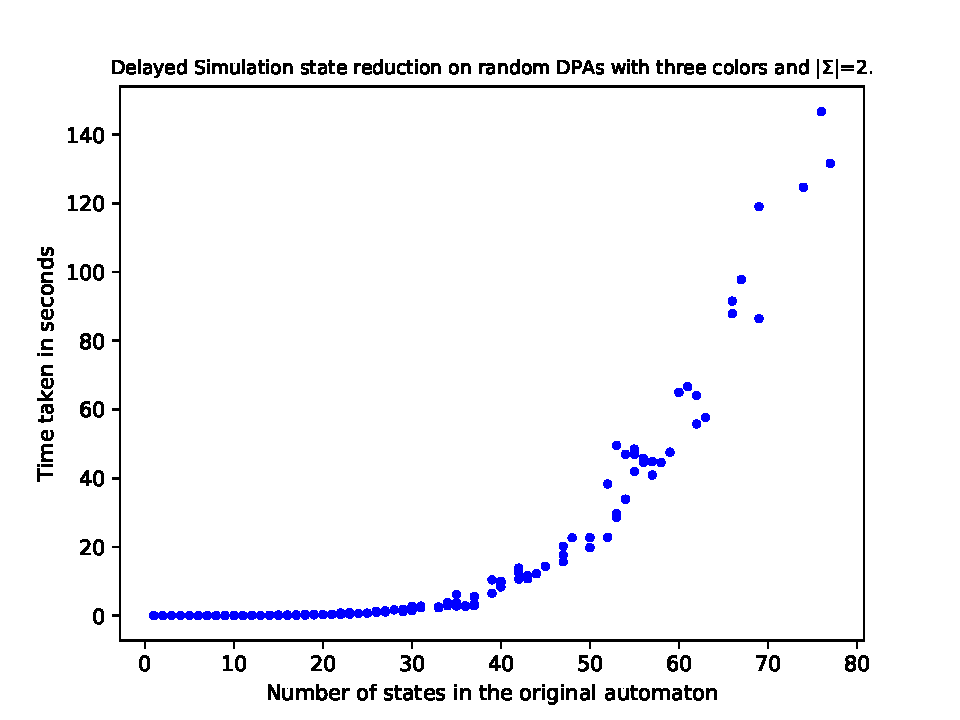
\includegraphics[page=1,height=.3\textheight]{../data/analysis/fritzwilke/gendet_ap1.pdf} 
	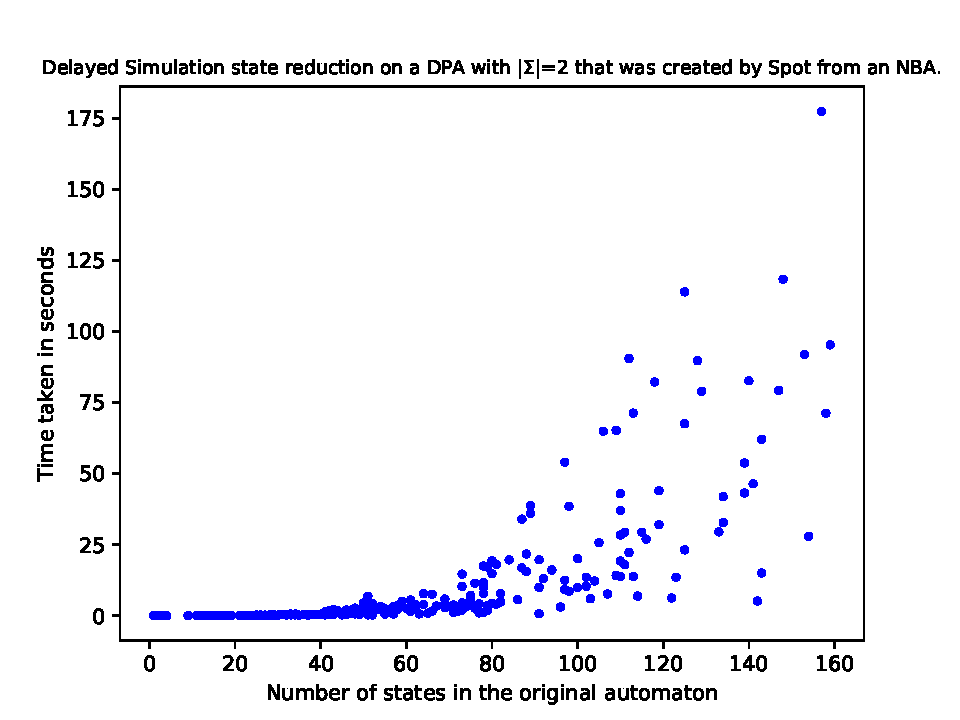
\includegraphics[page=1,height=.3\textheight]{../data/analysis/fritzwilke/detspot_ap1.pdf} 
	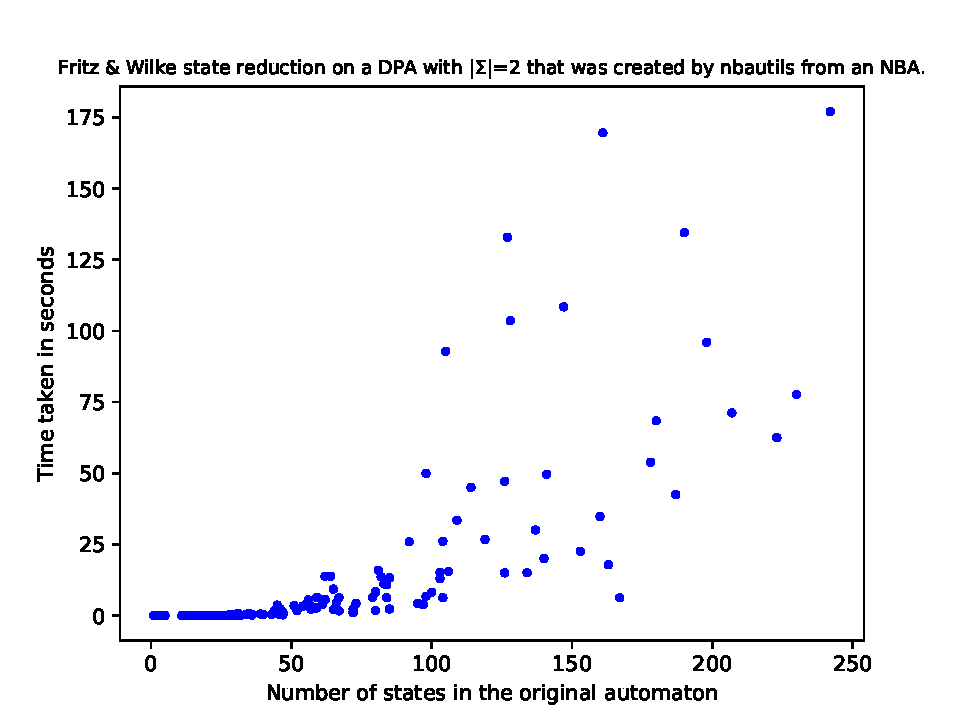
\includegraphics[page=1,height=.3\textheight]{../data/analysis/fritzwilke/detnbaut_ap1.pdf} 
	\caption{Run time of delayed simulation.}
	\label{exp:fig:fritzwilke_time}
\end{figure}